\documentclass[11pt,a4paper]{article}
\usepackage[T1]{fontenc}
\usepackage[utf8]{inputenc}
\usepackage{lmodern}
\usepackage[a4paper,margin=2.4cm]{geometry}
\usepackage{amsmath,amssymb}
\usepackage{graphicx}
\usepackage{booktabs,tabularx,array}
\usepackage{float}
\usepackage{microtype}
\usepackage{enumitem}
\usepackage[font=small,labelfont=bf,labelsep=period]{caption}
\usepackage[colorlinks=true,linkcolor=black,urlcolor=black,citecolor=black]{hyperref}
\setlength{\parskip}{0.55em}
\setlength{\parindent}{0pt}
\setlength{\emergencystretch}{3em}
\setlist{itemsep=0.2em,topsep=0.3em}
\renewcommand{\arraystretch}{1.15}
\setkeys{Gin}{keepaspectratio}
\title{\textbf{Inverse Problems with Multiple Valid Solutions:\\[0.2em] Mixture Density Networks for a Non-Injective Forward Map}}
\author{}
\date{}
\hypersetup{pdftitle={Inverse Problems with Multiple Valid Solutions: Mixture Density Networks for a Non-Injective Forward Map},pdfauthor={MAC 312 Project 8 group}}

\begin{document}
\maketitle
\vspace{-2.5em}
\begin{center}\large MAC 312 Foundations of Data Science \textperiodcentered{} Project 8\end{center}

\begin{table}[H]
\centering\small
\begin{tabular}{ll}
\toprule
\textbf{Name} & \textbf{ID number} \\
\midrule
Aamil Finoj & 2024ADPS0873G \\
Ashwath Chandramouli & 2024ADPS0853G \\
Advay Satish & 2024ADPS0826G \\
Arnav Kulshreshtha & 2024ADPS0821G \\
Rohan Agrawal & 2024ADPS0004G \\
Joel Thomas Thomas & 2024ADPS0848G \\
\bottomrule
\end{tabular}
\end{table}

\section*{Summary}
A mixture density network (MDN) recovers every valid answer of an ambiguous inverse problem, and a network trained with squared error cannot: on held-out data the MDN sits 0.03 nats above the exact posterior, against 1.68 nats for a single Gaussian.

We study the inverse of $x = t^{2} + \varepsilon$. Squaring discards the sign of $t$, so an observation $x$ is explained by two values, +$\sqrt{x}$ and $-\sqrt{x}$. Because the forward map is known, we can compute the exact posterior $p(t \mid  x)$ by numerical integration and grade every model against it, instead of judging plots by eye. We trained about 265 small networks to test three things: whether point estimators fail, whether an MDN finds both answers, and how far the MDN holds up under rare answers, small samples and noise.

\begin{itemize}
\item \textbf{Point estimators answer a different question.} The MSE network reaches the Bayes-optimal MSE (1.339, the same as the exact posterior) while predicting about 0, a value that is never a valid answer. An absolute-error (MAE) network learns the median, which picks one branch or wanders in the gap.
\item \textbf{The MDN matches the exact posterior.} With $M = 3$ components the excess negative log-likelihood (NLL) is 0.030 $\pm$ 0.007 and the Wasserstein-1 distance 0.040. 94\% of forward residuals fall within $\pm 2\sigma$, against 95\% for the true noise. Its calibration (PIT KS distance 0.013) matches the exact posterior (0.012).
\item \textbf{Rare answers survive.} With prior weight $q = 0.97$ on $t > 0$ (about 300 training points on the minority branch), every MDN with $M \ge  2$ recovered the rare branch in 60 of 60 runs. The single Gaussian never did.
\item \textbf{Failure has a precise location.} Recovery breaks only with about 10 minority training points, or with a variance floor wider than the true branch width (floor 0.1: capture 0.43).
\item \textbf{Remaining error is structural.} It sits where the true posterior has features a Gaussian mixture cannot draw: the hard edge at $\pm$a, the prior's jump at $t = 0$, and very sharp peaks at low noise. A truncated-component MDN removes the edge error (excess NLL 0.018, zero leaked mass).
\end{itemize}

Every number in this report is read from the saved result tables in the project repository and was cross-checked against them before submission.

\section{Problem and setup}
The forward map $t \to  t^{2}$ is not injective, so the inverse problem has no unique solution: the right object to estimate is the conditional distribution $p(t \mid  x)$, not a function $x \to  t$.

\textbf{The game, in plain terms.} Pick a secret number between $-$2 and 2, square it, add a small random wobble and report the result. If the report is 1, the secret was either +1 or $-$1, because squaring threw the sign away. A model that must return one number is punished least by guessing the middle, 0, and 0$^{2}$ = 0 is not 1. It always answers with something that is never a right answer.

\textbf{The generative model.}

\[
t \sim \mathrm{Unif}[-a,a], \qquad x = t^2 + \epsilon, \qquad \epsilon \sim \mathcal{N}(0,\sigma^2)
\]

The baseline uses $a = 2$ and $\sigma  = 0.15$. Data are fixed by \texttt{data\_\allowbreak{}seed = 2026}: 10,000 training, 2,000 validation and 2,000 test points. The test set is used only for reporting.

\textbf{The asymmetric prior.} To make the problem harder we also draw $t$ from a prior that puts weight $q$ on $t > 0$ and $1 - q$ on $t < 0$ ($q = 0.5$ is the symmetric baseline). The likelihood depends only on $t^{2}$, so $P(t > 0 \mid  x) = q$ exactly, for every $x$. This gives the imbalance experiments a known target: a model that recovers the rare branch must put mass $1 - q$ (or $q$) on it at every input.

\textbf{Why the task is non-trivial.} The forward model is easy to simulate, so data are unlimited and noise is controlled. What makes it hard is that the quantity of interest is a multimodal distribution, and the usual training recipe (minimise squared error) estimates only its mean.

\section{The exact posterior as ground truth}
Because the noise model is known, Bayes' rule gives $p(t \mid  x)$ in closed form up to one integral, so every trained model can be scored against the truth rather than against another model.

\[
p(t\mid x)=\frac{\exp\!\big[-\tfrac{(x-t^2)^2}{2\sigma^2}\big]}{Z(x)}\,\mathbb{1}_{[-a,a]}(t),\qquad Z(x)=\int_{-a}^{a} e^{-(x-u^2)^2/2\sigma^2}\,du
\]

$Z(x)$ has no elementary closed form, so we compute it with \texttt{scipy.integrate.quad}. Three choices keep it stable:

\begin{itemize}
\item subtract the maximum of the log-integrand before exponentiating;
\item split the integral at $t = 0$;
\item pass the peak locations $\pm \sqrt{x}$ to the integrator as break points.
\end{itemize}

The integrand is even in $t$, so the two half-integrals are equal under the symmetric prior. With the asymmetric prior only the prior weights (2q and $2(1 - q)$) differ, which is why $P(t > 0 \mid  x) = q$ holds exactly. The posterior mean is $E[t \mid  x] = (2q - 1)$ times the half-mean. Half-integrals are cached, so repeated evaluations are cheap.

\textbf{Where the solutions are.} The derivative of log p is 2t($x - t^{2}$)/$\sigma ^{2}$, so the stationary points are $t = 0$ and $t$ = $\pm \sqrt{x}$. For $x > 0$ the point $t = 0$ is a local minimum of log p (curvature 2x/$\sigma ^{2}$), and each branch has local standard deviation $\sigma$/($2\sqrt{x}$). For $0 < x \le  a^{2}$ the valley-to-peak density ratio is $\exp(-x^{2}/2\sigma ^{2})$; beyond $a^{2}$ the peaks sit at $\pm$a instead. This gives four input regions, used later to locate where each model loses accuracy:

\begin{table}[H]
\centering\small
\begin{tabularx}{\linewidth}{ll>{\raggedright\arraybackslash}X}
\toprule
\textbf{Region} & \textbf{$x$} & \textbf{Posterior shape} \\
\midrule
No real inverse & $x \le  0$ & One mode at $t = 0$ \\
Merged & $0 < x < 2\sigma$ & Two modes, barely separated \\
Two branches & $2\sigma  \le  x \le  a^{2}$ & Clear modes at $\pm \sqrt{x}$ \\
Beyond support & $x > a^{2}$ & Modes pinned to $\pm$a by the prior \\
\bottomrule
\end{tabularx}
\end{table}

\textbf{How we know the reference is right.} The notebook checks that the density integrates to 1, is symmetric, and does not change with the integration tolerance or against a 400,001-point grid. A separate standalone test file (\texttt{tests/\allowbreak{}test\_\allowbreak{}reference.py}, 71 checks) compares the reference against an independent midpoint-rule grid. It covers normalisation, $P(t > 0 \mid  x) = q$ for $q = 0.5$ and 0.9, the posterior mean, symmetry, the modes and regions, the valley/peak ratio, edge cases ($\sigma  = 0.05$ and 0.5, $q = 0$, 0.5 and 1, $x$ from $-$5 to 10) and rejection of invalid parameters. All 71 pass, and the tests treat any numerical warning as an error.

\section{Why standard regression fails}
A point estimator returns one summary of $p(t \mid  x)$, and for a two-peaked posterior every common summary lands in the wrong place. Squared loss returns the mean, and absolute loss returns the median.

\textbf{The MSE network.} It outputs one number $f(x)$ and minimises the average squared error. The expected loss splits into two terms:

\[
\mathbb{E}\big[(f-t)^2\big]=\mathbb{E}\big[(f-\mathbb{E}[t\mid x])^2\big]+\mathbb{E}\big[\mathrm{Var}(t\mid x)\big]
\]

The second term does not depend on $f$, so the optimum is the conditional mean $E[t \mid  x]$. Under the symmetric prior this is 0 everywhere, exactly between the two branches. Under $q = 0.9$ it is about $(2q - 1)\sqrt{x} = 0.8\sqrt{x}$, which is still not on a branch.

Our network reached the Bayes-optimal value: test MSE 1.3388 against 1.3386 for the exact conditional mean. It is a perfect estimator of a summary that is useless for this problem. The forward check shows it: squaring its prediction misses the observation by a mean absolute error of 2.15, and only 26\% of its forward residuals fall within $\pm 2\sigma$ (residual sd 1.198 against the true noise sd 0.15).

\begin{figure}[H]
\centering
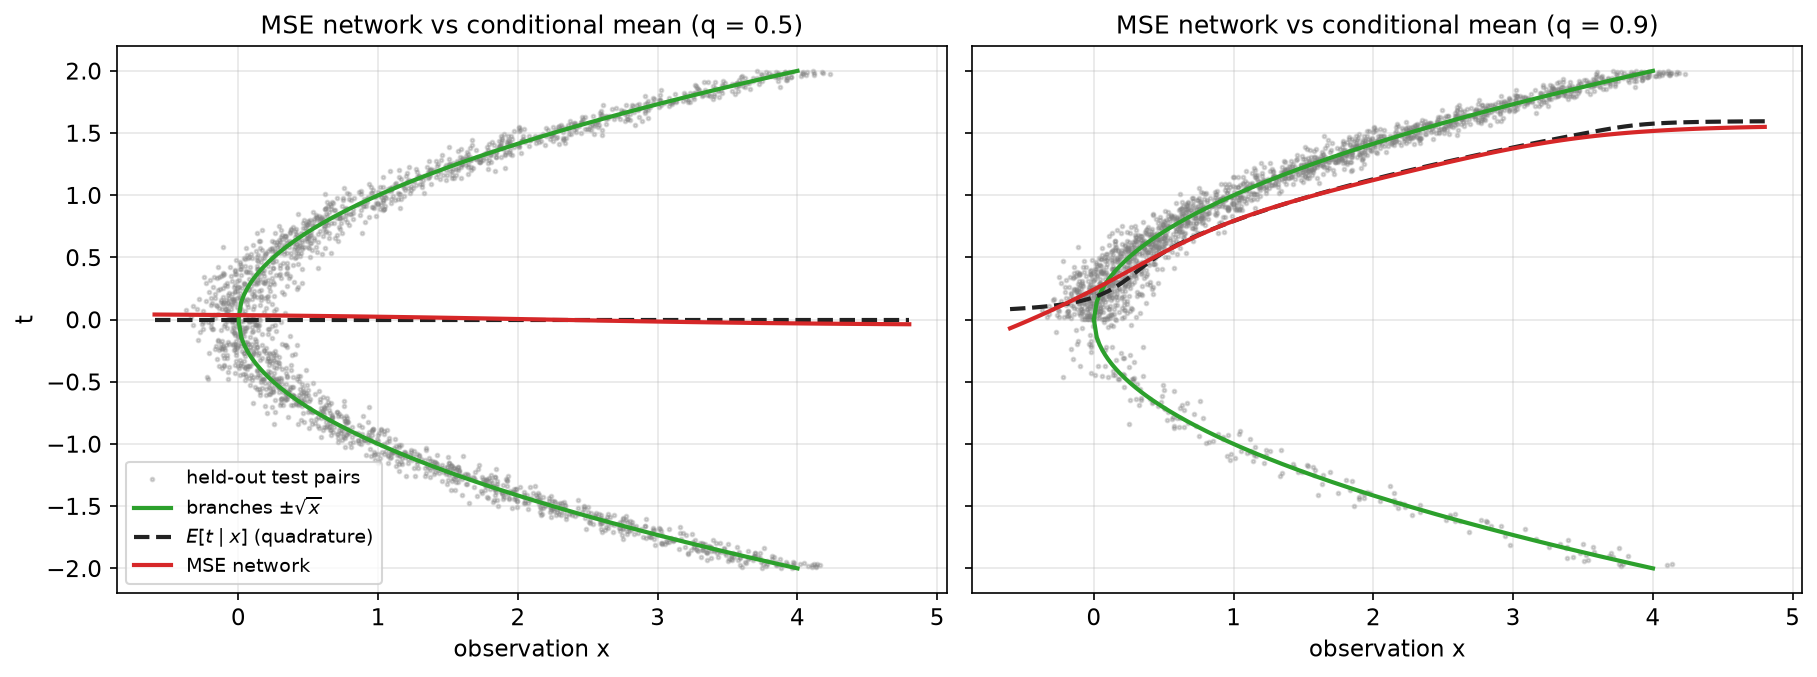
\includegraphics[width=\linewidth]{figures/mse_predictions.png}
\caption{The MSE network (red) tracks the conditional mean (dashed) almost exactly. For $q = 0.5$ it runs along $t = 0$, between the two branches (green); for $q = 0.9$ it runs below the majority branch. Grey points are held-out test pairs.}
\end{figure}

\textbf{The MAE network.} The same network trained with absolute error learns the conditional median.

\begin{table}[H]
\centering\small
\begin{tabularx}{\linewidth}{lll>{\raggedright\arraybackslash}X>{\raggedright\arraybackslash}X}
\toprule
\textbf{Prior} & \textbf{Loss} & \textbf{Test MSE} & \textbf{Share of predictions near +branch} & \textbf{Share in the gap} \\
\midrule
$q = 0.5$ & MSE & 1.339 & 0.00 & 1.00 \\
$q = 0.5$ & MAE (5 seeds) & 2.15 to 2.33 & 0.21 to 0.34 & 0.66 to 0.79 \\
$q = 0.9$ & MSE & 0.475 & 0.22 & 0.78 \\
$q = 0.9$ & MAE (5 seeds) & 0.518 to 0.523 & 1.00 & 0.00 \\
$q = 0.9$ & exact median & 0.519 & n/a & n/a \\
\bottomrule
\end{tabularx}
\end{table}

Under $q = 0.9$ the median lands on the majority branch every time: a valid answer, but only one of the two, and the minority branch is invisible. Under the symmetric prior the median is 0, but the absolute loss is almost flat across the whole gap, so the trained networks wander inside it and partly drift onto the positive branch (following a 50.8\% sign imbalance in the training sample).

\textbf{The point.} Changing the point loss changes which single answer you get, never the fact that you get only one. Maximum likelihood on a flexible density is the natural fix: it minimises KL(p \textbar{}\textbar{} p\_$\theta$), which punishes a model heavily for leaving any true branch with no mass.

\section{Mixture density networks}
An MDN outputs a probability distribution instead of a number: a mixture of $M$ Gaussians whose weights, means and variances all depend on $x$.

\[
p_\theta(t\mid x)=\sum_{j=1}^{M}\pi_j(x)\,\mathcal{N}\big(t\mid \mu_j(x),v_j(x)\big),\qquad \pi=\mathrm{softmax}(\alpha),\quad v_j=\mathrm{softplus}(s_j)+v_{\min}
\]

The softmax makes the weights positive and sum to 1, and the softplus plus a floor makes every variance positive, so the output is a valid density by construction. The floor v\_min = 10$^{-4}$ is a variance floor.

\textbf{Architecture and training (all networks).} One shared small trunk: 1 input (standardised $x$), 3 hidden layers of 64 tanh units. Adam with learning rate 2$\times$10$^{-3}$, batch size 256, gradient clipping at norm 5, up to 400 epochs, and early stopping on the validation loss (patience 40) with the best checkpoint restored. The test set never influences training.

\textbf{The single Gaussian is the MDN with $M = 1$}, using the same code with a different $M$. It models uncertainty but has only one bump.

\textbf{The loss, in log space.} Training minimises the average negative log-likelihood, computed with the log-sum-exp trick:

\[
-\log p=-\operatorname{logsumexp}_j\Big[\log\pi_j-\tfrac12\log(2\pi v_j)-\tfrac{(t-\mu_j)^2}{2v_j}\Big]
\]

The naive version, summing the densities and then taking a log, underflows. At $t = 30$ it returns $-$$\infty$, whereas log-sum-exp returns a finite value ($-$3105 in the notebook demonstration), and gradients stay finite.

\textbf{Truncated MDN (extension).} A Gaussian mixture has unbounded support, but the true posterior lives on [$-$a, a]. In the truncated variant each component is a Gaussian truncated to [$-$a, a] and renormalised, so no mass leaks outside the support and samples are guaranteed to lie inside it. It is selected with \texttt{MDNConfig(truncate=True)}.

\textbf{What we verify about the MDN.} \texttt{tests/\allowbreak{}test\_\allowbreak{}mdn.py} (16 checks) confirms the weights sum to 1, variances stay above the floor, the log-probability matches SciPy, the naive version underflows at $t = 30$ while log-sum-exp stays finite with finite gradients, the truncated density integrates to 1 on [$-$a, a] with zero out-of-support mass and $-$$\infty$ log-probability outside it, branch probability and mean match a grid computation, samples stay inside the support, and a short training run stays finite. All 16 pass on the standard and truncated models.

\section{Evaluation metrics and experimental design}
Because the exact posterior is known, each metric measures distance to the truth, and each one answers a different question.

\begin{table}[H]
\centering\small
\begin{tabularx}{\linewidth}{l>{\raggedright\arraybackslash}X>{\raggedright\arraybackslash}X}
\toprule
\textbf{Metric} & \textbf{Definition} & \textbf{What it tells us} \\
\midrule
Excess NLL & Test NLL of the model minus test NLL of the exact posterior & Estimates the average KL divergence from truth to model. 0 is perfect \\
Branch-probability error & Absolute difference between the model's $P(t > 0 \mid  x)$ and $q$ & Is the sign split right? \\
Branch capture and recovery & Model mass divided by reference mass within $\pm \sqrt{x}$ $\pm$ $3\sigma$/($2\sqrt{x}$), scored where two modes exist ($2\sigma  \le  x \le  a^{2} - 2\sigma$). A branch is recovered if capture $\ge$ 0.5 & Measures branches by probability mass, not by counting mixture components \\
Wasserstein-1 (W1) & Both densities on a common 4001-point grid, \texttt{scipy.stats.wasserstein\_\allowbreak{}distance} & How far mass is misplaced, in units of $t$ \\
Forward residual & r = $x - \tilde{t}^{2}$ with $\tilde{t}$ sampled from the model & If the model is exact, r has sd $\sigma$. The target is $\sigma$, not 0, because the data are noisy \\
PIT KS distance & Kolmogorov--Smirnov distance of the probability-integral transform from uniform & 0 means the predicted distribution is calibrated \\
Out-of-support mass & Model mass outside [$-$a, a] & A Gaussian mixture leaks some mass; truncation removes it \\
\bottomrule
\end{tabularx}
\end{table}

Two cautions about the metrics. First, mixture components are not modes, so we count recovery by probability mass in the neighbourhood of each branch. Second, the capture $\ge$ 0.5 threshold is our own and deliberately lenient, so the raw capture values are reported too. Grid-based metrics (W1, capture) truncate the model to [$-$a, a]; the leaked mass is reported separately.

\textbf{Experimental design.} Overlapping settings are trained once and reused. The dataset is fixed by \texttt{data\_\allowbreak{}seed}, so only the initialisation seed varies (seeds 0 to 4), and the spread across seeds isolates optimisation randomness. Python, NumPy and PyTorch are all seeded, and all settings are saved to \texttt{artifacts/\allowbreak{}results/\allowbreak{}settings.json}. In total the study trains about 265 distinct networks:

\begin{table}[H]
\centering\small
\begin{tabularx}{\linewidth}{l>{\raggedright\arraybackslash}Xl}
\toprule
\textbf{Experiment} & \textbf{What varies} & \textbf{Runs} \\
\midrule
Baseline & $M$ in \{1, 2, 3, 5\}, 5 seeds & 20 \\
Asymmetric prior & $q$ in \{0.5, 0.7, 0.9, 0.97\} $\times$ $M \times  5$ seeds & 80 \\
Initialisation & default vs spread starting means, $q$ in \{0.9, 0.97\}, $M$ in \{2, 3\} & 40 \\
Variance floor & floor in \{10$^{-5}$, ..., 10$^{-1}$\}, $q = 0.9$ & 25 \\
Noise robustness & $\sigma$ in \{0.05, 0.15, 0.3, 0.5\} $\times$ $q$ in \{0.5, 0.9\} $\times$ $M$ in \{1, 3\} & 80 \\
MSE networks & $q$ in \{0.5, 0.9\} & 2 \\
MAE (median) networks & $q$ in \{0.5, 0.9\} $\times$ 5 seeds & 10 \\
Truncated MDN & standard vs truncated components, $M = 3$, 5 seeds & 5 new \\
Sample size & N in \{1000, 2500, 10000\} $\times$ $q$ in \{0.9, 0.97, 0.99\}, plus spread init at $q = 0.99$, 5 seeds & 50 new \\
Prior jump at $t = 0$ & $M$ in \{5, 8\} at $\sigma  = 0.5$, $q$ in \{0.5, 0.9\}, 5 seeds (rest reused from the noise sweep) & 20 new \\
\bottomrule
\end{tabularx}
\end{table}

\section{Baseline results (symmetric prior, $\sigma  = 0.15$)}
All four models have essentially the same test MSE, but only the MDN has the right distribution: its excess NLL is 0.03 against 1.68 for the single Gaussian.

\begin{table}[H]
\centering\small
\begin{tabularx}{\linewidth}{lll>{\raggedright\arraybackslash}X>{\raggedright\arraybackslash}Xl}
\toprule
\textbf{Model} & \textbf{Excess NLL (1)} & \textbf{W1 (1)} & \textbf{Residuals within $\pm 2\sigma$ (2)} & \textbf{PIT KS distance (2)} & \textbf{Test MSE (2)} \\
\midrule
MSE network & n/a & n/a & 0.26 & n/a & 1.339 \\
Single Gaussian $(M = 1)$ & 1.68 & 0.45 & 0.35 & 0.24 & 1.339 \\
MDN $(M = 3)$ & 0.03 & 0.04 & 0.94 & 0.013 & 1.338 \\
Exact posterior & 0 & 0 & 0.96 & 0.012 & 1.339 \\
\bottomrule
\end{tabularx}
\end{table}

(1) Mean over 5 seeds. (2) Seed-0 model on the held-out test set, with 20 posterior samples per observation for the residuals. Test MSE is also the seed-0 model; the 5-seed mean for $M = 3$ is 1.341. For reference, the true noise itself has 95.1\% of residuals within $\pm 2\sigma$.

\begin{figure}[H]
\centering
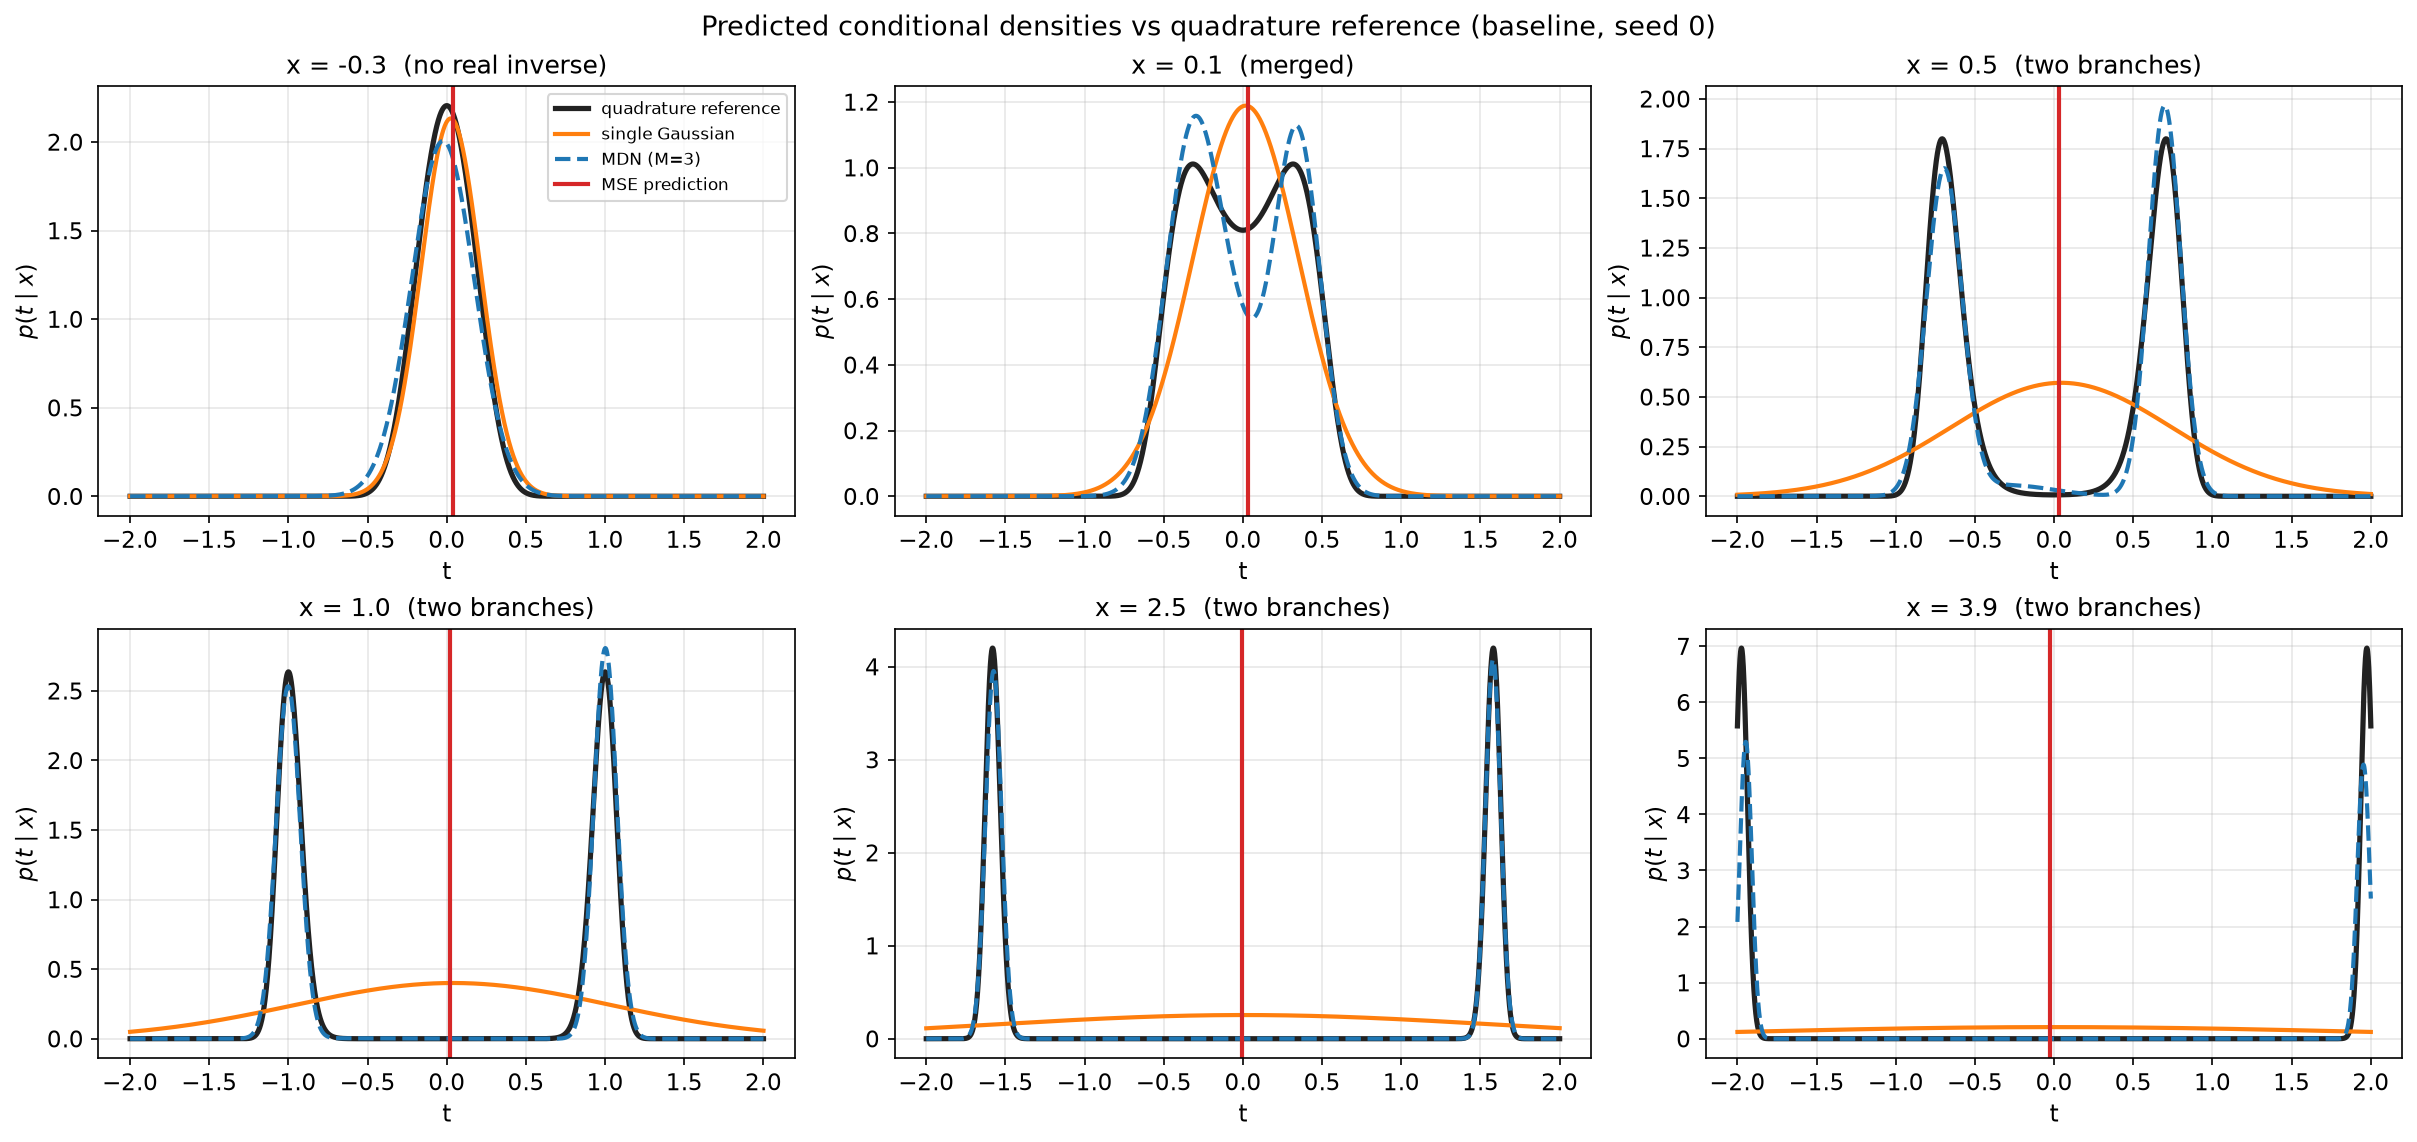
\includegraphics[width=\linewidth]{figures/density_comparison.png}
\caption{Predicted densities at six inputs (baseline, seed 0). Black: exact posterior. Blue dashed: MDN with $M = 3$, which tracks both peaks. Orange: single Gaussian, which spreads one wide bump over both branches. Red line: MSE prediction, at $t \approx  0$. The MDN's weak spots are visible at $x = 0.1$, where it over-draws the dip, and at $x = 3.9$, where it cannot reproduce the hard edge at $\pm$2.}
\end{figure}

\textbf{Reading the table.}

\begin{itemize}
\item The MSE column cannot tell the models apart. A model can have the best possible MSE and still be useless as an inverse, which is why we grade with likelihood-based metrics.
\item The single Gaussian is a bad answer in a specific way. With one bump it must either sit between the branches or cover both with a very wide spread. Its forward residuals have sd 2.47 against the true 0.15.
\item The MDN's forward residuals have sd 0.156 and 94.4\% fall within $\pm 2\sigma$, which is what an exact posterior would give.
\item Branch probability is about 0.5 for both probabilistic models, so a correct sign split does not imply a correct density: the single Gaussian gets the sign split right and the shape wrong.
\end{itemize}

\textbf{Choosing $M$.} Excess NLL by number of components, mean over 5 seeds:

\begin{table}[H]
\centering\small
\begin{tabular}{lllll}
\toprule
\textbf{$M$} & \textbf{Excess NLL} & \textbf{Seed sd} & \textbf{W1} & \textbf{Out-of-support mass} \\
\midrule
1 & 1.678 & 0.0005 & 0.448 & 0.094 \\
2 & 0.027 & 0.004 & 0.036 & 0.009 \\
3 & 0.030 & 0.007 & 0.040 & 0.007 \\
5 & 0.027 & 0.006 & 0.047 & 0.008 \\
\bottomrule
\end{tabular}
\end{table}

On validation NLL any $M \ge  2$ is as good as any other ($M = 2$, 3, 5 are within one seed sd), so $M = 3$ is a safe choice, not a tuned optimum.

\textbf{Where the remaining error sits.} Splitting the test set into the four input regions of section 2 shows that the single Gaussian's error is almost entirely in the two-branch region (95\% of its excess NLL, 2.19 nats per point there). The MDN's small residual error is spread more evenly:

\begin{table}[H]
\centering\small
\begin{tabular}{lll}
\toprule
\textbf{Region (test points)} & \textbf{MDN excess NLL} & \textbf{Share of MDN total} \\
\midrule
No real inverse (178) & 0.024 & 8\% \\
Merged (341) & 0.013 & 8\% \\
Two branches (1459) & 0.022 & 60\% \\
Beyond support (22) & 0.592 & 24\% \\
\bottomrule
\end{tabular}
\end{table}

About a quarter of the MDN's small excess NLL comes from the 1\% of test points beyond the support ($x > a^{2}$), where a Gaussian mixture cannot draw the hard edge at $\pm$a. That motivates the truncated MDN of section 8.

\section{Imbalanced prior: does the rare answer survive?}
Every MDN with $M \ge  2$ recovered the rare branch in 60 of 60 runs, even at a 97:3 split where only about 300 training points lie on it; the single Gaussian did not. Here $q$ is the prior weight on $t > 0$, and the minority branch is the one with weight $1 - q$.

\begin{table}[H]
\centering\small
\begin{tabular}{lllll}
\toprule
\textbf{$q$} & \textbf{$M$} & \textbf{Minority capture} & \textbf{Recovered fraction of inputs} & \textbf{Excess NLL} \\
\midrule
0.7 & 1 & 0.16 & 0.05 & 1.681 \\
0.7 & 2 & 0.94 & 1.00 & 0.037 \\
0.7 & 3 & 0.98 & 1.00 & 0.032 \\
0.7 & 5 & 0.92 & 1.00 & 0.033 \\
0.9 & 1 & 0.05 & 0.01 & 1.594 \\
0.9 & 2 & 0.92 & 1.00 & 0.035 \\
0.9 & 3 & 0.92 & 1.00 & 0.035 \\
0.9 & 5 & 1.00 & 1.00 & 0.038 \\
0.97 & 1 & 0.01 & 0.00 & 1.357 \\
0.97 & 2 & 1.01 & 1.00 & 0.051 \\
0.97 & 3 & 0.91 & 1.00 & 0.042 \\
0.97 & 5 & 0.91 & 1.00 & 0.046 \\
\bottomrule
\end{tabular}
\end{table}

Mean over 5 seeds. Capture is model mass divided by reference mass on the minority branch (1 is perfect).

\begin{figure}[H]
\centering
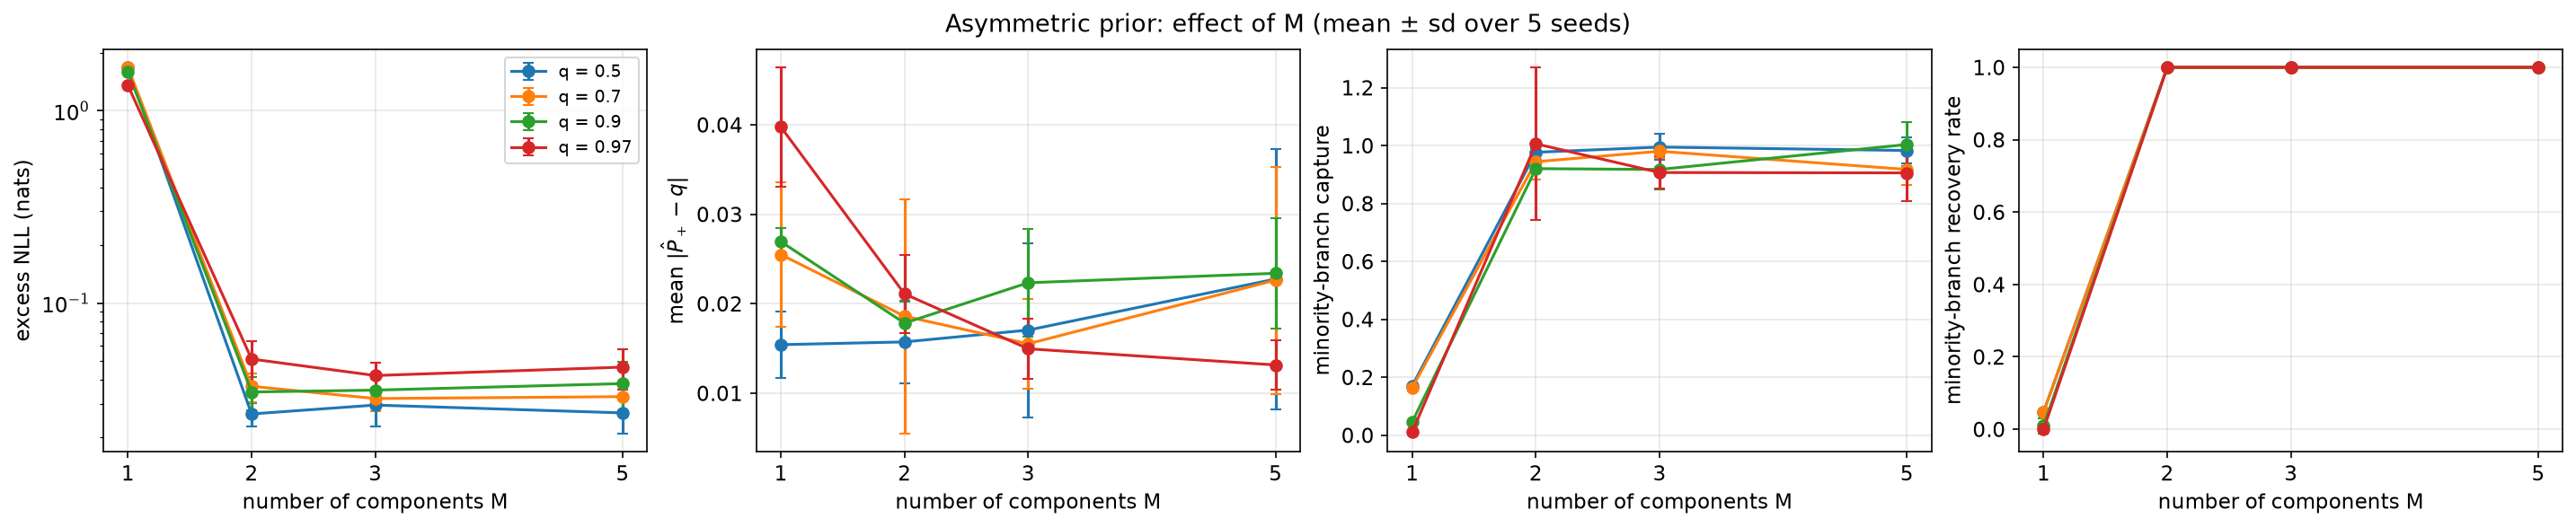
\includegraphics[width=\linewidth]{figures/asym_vs_M.png}
\caption{Effect of the number of components $M$ for $q = 0.5$, 0.7, 0.9 and 0.97 (mean $\pm$ sd over 5 seeds). Going from $M = 1$ to $M = 2$ collapses the excess NLL from about 1.5 to about 0.03 and lifts minority capture and the recovery rate to about 1; further components change little.}
\end{figure}

\textbf{Findings.}

\begin{itemize}
\item \textbf{$M = 1$ cannot recover the rare branch, whatever the seed.} This is a capacity limit, not a training problem: one Gaussian has no way to place mass on two separate branches.
\item \textbf{Recovery is not perfect.} Minority capture drops from about 0.97 at $q = 0.5$ to about 0.94 at $q = 0.97$ (the rare branch is slightly under-weighted), and variation across seeds grows with the imbalance. The sd of minority capture over seeds is about 0.03 at $q = 0.5$, 0.07 at $q = 0.9$ and 0.16 at $q = 0.97$ $(M \ge  2)$.
\item \textbf{MSE cannot see any of this.} At $q = 0.9$ the test MSE is about 0.473 to 0.474 for every $M$, while the excess NLL ranges from 0.035 to 1.6.
\item \textbf{Branch-probability error stays small} (about 0.013 to 0.04) across all of the above, so the sign split is learned even when branch shape is imperfect.
\end{itemize}

\textbf{Initialisation.} We compared PyTorch default starting means against a "spread" start that places component means across [$-$a, a]. At N = 10,000 and $q \le  0.97$, initialisation and $M > 2$ hardly matter:

\begin{table}[H]
\centering\small
\begin{tabularx}{\linewidth}{ll>{\raggedright\arraybackslash}X>{\raggedright\arraybackslash}X}
\toprule
\textbf{$q$} & \textbf{$M$} & \textbf{Default init: capture / excess NLL} & \textbf{Spread init: capture / excess NLL} \\
\midrule
0.9 & 2 & 0.92 / 0.035 & 0.92 / 0.042 \\
0.9 & 3 & 0.92 / 0.035 & 0.88 / 0.031 \\
0.97 & 2 & 1.01 / 0.051 & 1.00 / 0.049 \\
0.97 & 3 & 0.91 / 0.042 & 0.92 / 0.047 \\
\bottomrule
\end{tabularx}
\end{table}

\textbf{Variance floor.} What does break recovery is a floor wider than the true branch width. At $q = 0.9$, $M = 3$:

\begin{table}[H]
\centering\small
\begin{tabular}{lll}
\toprule
\textbf{Variance floor} & \textbf{Minority capture} & \textbf{Excess NLL} \\
\midrule
10$^{-5}$ & 0.94 & 0.040 \\
10$^{-4}$ & 0.92 & 0.035 \\
10$^{-3}$ & 0.97 & 0.038 \\
10$^{-2}$ & 0.91 & 0.185 \\
10$^{-1}$ & 0.43 & 0.909 \\
\bottomrule
\end{tabular}
\end{table}

A variance floor of 0.1 forces every component to have sd of at least 0.32, many times the true branch sd (about 0.04 to 0.08 for $x$ between 4 and 1 at $\sigma  = 0.15$), so the rare branch is smeared and capture falls below 0.5. A floor of 0.01 (sd 0.1) keeps recovery but costs likelihood.

\textbf{Sample-size stress test.} To find where recovery actually breaks, we reduced the training set (N = 1000, 2500, 10000) and pushed $q$ to 0.99, with the step budget held fixed ($M = 3$, 5 seeds each):

\begin{table}[H]
\centering\small
\begin{tabularx}{\linewidth}{ll>{\raggedright\arraybackslash}X>{\raggedright\arraybackslash}X>{\raggedright\arraybackslash}X>{\raggedright\arraybackslash}X}
\toprule
\textbf{N} & \textbf{$q$} & \textbf{Minority training points} & \textbf{Capture (mean $\pm$ sd)} & \textbf{Recovered fraction} & \textbf{Seeds with capture \textless{} 0.5} \\
\midrule
1000 & 0.9 & 100 & 1.18 $\pm$ 0.07 & 1.00 & 0 of 5 \\
1000 & 0.97 & 30 & 1.23 $\pm$ 0.11 & 1.00 & 0 of 5 \\
1000 & 0.99 & 10 & 0.49 $\pm$ 0.23 & 0.46 & 2 of 5 \\
2500 & 0.99 & 25 & 1.06 $\pm$ 0.30 & 1.00 & 0 of 5 \\
10000 & 0.99 & 100 & 0.78 $\pm$ 0.20 & 0.77 & 0 of 5 \\
\bottomrule
\end{tabularx}
\end{table}

Capture above 1 means the model puts more mass on that branch than the reference does (a mild over-weighting). Down to about 30 minority points the rare branch is recovered on every seed. At about 10 minority points it breaks, and spread initialisation does not rescue it (capture 0.55, 1 of 5 seeds lost). The result at $q = 0.99$ is not monotone in N: N = 2500 recovers fully while N = 10,000 recovers only 77\% of the recovery grid. With a single dataset per N, we read this as variation between dataset draws and not as an effect of N. Spread initialisation did help at N = 10,000 (recovered fraction 0.77 to 0.99).

\begin{figure}[H]
\centering
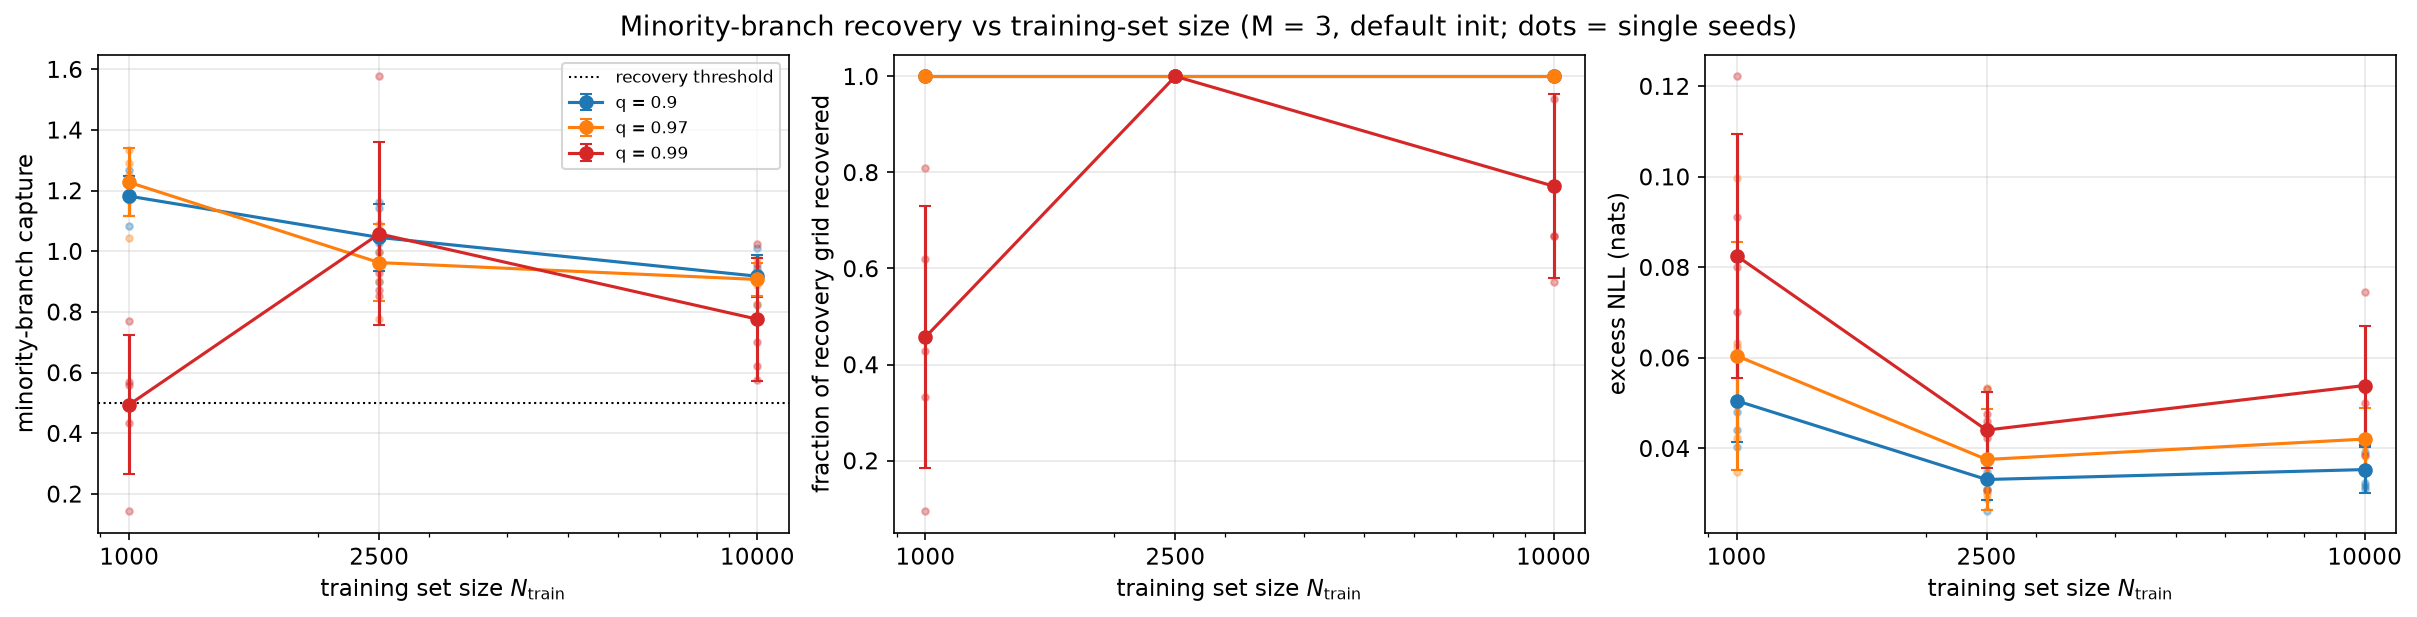
\includegraphics[width=\linewidth]{figures/sample_size_stress_test.png}
\caption{Sample-size stress test ($M = 3$, default initialisation; small dots are single seeds). Left: minority capture against the 0.5 recovery threshold. Middle: fraction of the recovery grid recovered. Right: excess NLL. The $q = 0.99$ curve at N = 1000 (about 10 minority points) is the only one that drops below the threshold.}
\end{figure}

\section{Extensions}
Three extensions test whether the MDN's remaining error has an identifiable cause and whether the conclusions hold when the noise level changes.

\subsection{Truncated MDN: removing the support-edge error}
Truncating each component to [$-$a, a] removes the leaked mass and lowers the baseline excess NLL from 0.030 to 0.018 nats, better on every one of the 5 seeds. Its W1 is not better, because W1 already truncates the standard MDN before comparing.

\begin{table}[H]
\centering\small
\begin{tabularx}{\linewidth}{lll>{\raggedright\arraybackslash}X>{\raggedright\arraybackslash}X}
\toprule
\textbf{$M = 3$, 5 seeds} & \textbf{Excess NLL} & \textbf{W1} & \textbf{Out-of-support mass} & \textbf{Branch-probability error} \\
\midrule
Standard MDN & 0.030 $\pm$ 0.007 & 0.040 $\pm$ 0.022 & 0.0065 & 0.017 \\
Truncated MDN & 0.018 $\pm$ 0.006 & 0.048 $\pm$ 0.026 & 0.0000 & 0.024 \\
\bottomrule
\end{tabularx}
\end{table}

The gain matches the region analysis in section 6: the largest per-point error of the standard MDN is beyond the support, exactly where truncation helps.

\subsection{Noise robustness}
Both branches were recovered at every noise level from $\sigma  = 0.05$ to 0.5. Excess NLL, mean over 5 seeds:

\begin{table}[H]
\centering\small
\begin{tabularx}{\linewidth}{l>{\raggedright\arraybackslash}X>{\raggedright\arraybackslash}X>{\raggedright\arraybackslash}X>{\raggedright\arraybackslash}X}
\toprule
\textbf{$\sigma$} & \textbf{Single Gaussian $(q = 0.9)$} & \textbf{MDN $M = 3$ $(q = 0.5)$} & \textbf{MDN $M = 3$ $(q = 0.9)$} & \textbf{MDN minority capture $(q = 0.9)$} \\
\midrule
0.05 & 2.494 & 0.051 & 0.091 & 0.95 \\
0.15 & 1.594 & 0.030 & 0.035 & 0.92 \\
0.30 & 1.088 & 0.025 & 0.032 & 0.96 \\
0.50 & 0.771 & 0.030 & 0.028 & 0.90 \\
\bottomrule
\end{tabularx}
\end{table}

\begin{itemize}
\item \textbf{The MDN's error is worst at the smallest noise} (0.09 at $\sigma  = 0.05$ with $q = 0.9$). The branches become very sharp (sd $\sigma$/($2\sqrt{x}$), about 0.0125 to 0.025 for $x$ between 4 and 1), and small width errors then cost a lot of log-likelihood.
\item \textbf{The single Gaussian looks relatively better at high noise} only because the true posterior itself becomes blurrier, so one bump is a less bad approximation. It is still more than 20 times worse than the MDN at every noise level.
\end{itemize}

\begin{figure}[H]
\centering
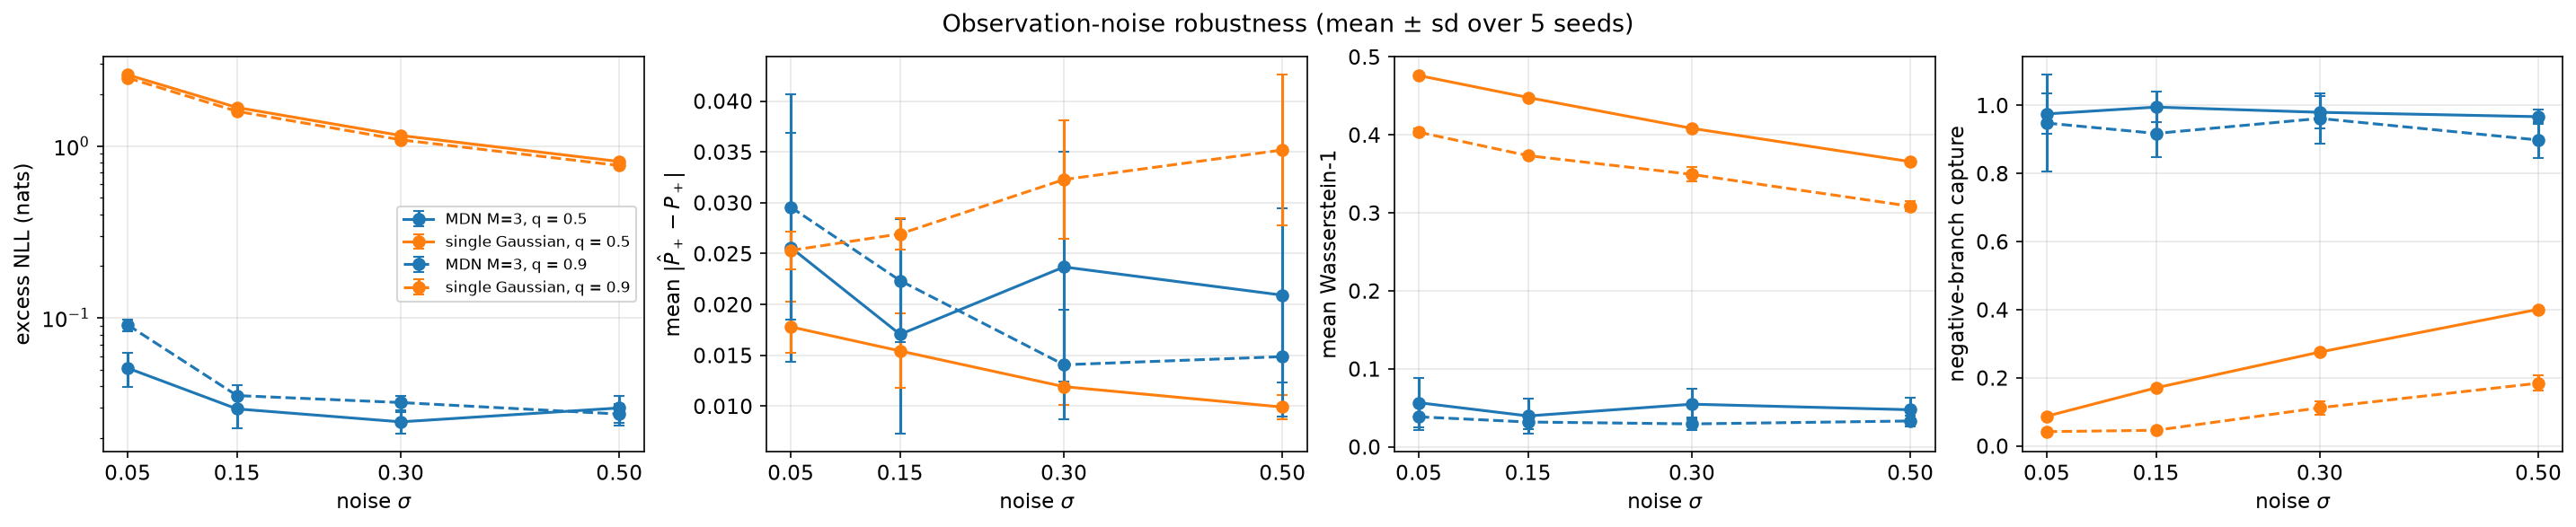
\includegraphics[width=\linewidth]{figures/noise_metrics.png}
\caption{Robustness to observation noise (mean $\pm$ sd over 5 seeds; solid $q = 0.5$, dashed $q = 0.9$). Blue: MDN with $M = 3$. Orange: single Gaussian. The MDN stays near 0.03 nats at every $\sigma$ except the smallest, while the single Gaussian's excess NLL stays above 0.7 and its capture of the second branch stays below 0.5.}
\end{figure}

\subsection{The prior's jump at $t = 0$}
With $q = 0.9$ the exact posterior has a step at $t = 0$ at every noise level, because $p(s \mid  x)$ / $p(-s \mid  x) = q$ / $(1 - q)$ for every s \textgreater{} 0: the density just right of 0 is nine times the density just left of it. Noise only changes how much of the input range shows this step: it is visible for 19\% of inputs at $\sigma  = 0.05$ and 51\% at $\sigma  = 0.5$.

A sum of smooth Gaussians cannot draw a step. The MDN draws a ramp about 0.1 to 0.2 wide in \textbar{}$t$\textbar{} (0.17 at $\sigma  = 0.05$, 0.14 at $\sigma  = 0.5$ for $M = 3$). This costs at most about 0.01 nats of NLL (0.002 at $\sigma  = 0.05$ up to 0.012 at $\sigma  = 0.5$), and it does not change branch probabilities or recovery. Going from $M = 3$ to $M = 8$ does not remove it (ramp width 0.14 at $M = 3$, 0.12 at $M = 8$, at $\sigma  = 0.5$). A separate sign model or a normalising flow would be the natural next step for the jump.

\section{Limitations}
The results are strong for this problem, but they are measured on a deliberately simple one, and several choices limit how far they generalise.

\begin{itemize}
\item \textbf{One architecture.} Every network is a 3 $\times$ 64 tanh MLP. We did not test wider, deeper or differently regularised networks.
\item \textbf{One training-set size, except in the stress test.} The main experiments use 10,000 training points. Smaller sizes appear only in the sample-size experiment, and much less data or more extreme imbalance than we tried may lose the rare branch (untested).
\item \textbf{One dataset per setting.} The notebook also runs on Google Colab: a setup cell at the top locates the repository (or unzips or clones it), changes into its folder and installs the missing packages. The data are fixed by \texttt{data\_\allowbreak{}seed}, and seeds vary only the initialisation. At very few minority points the draw of rare points and the effect of N cannot be separated, which is why the non-monotone result at $q = 0.99$ is read as dataset-draw variation.
\item \textbf{A lenient recovery threshold.} "Recovered" means capture $\ge$ 0.5, our own definition. We therefore report raw capture values too, and note that capture runs from about 0.9 to just over 1.0, so the rare branch is slightly under-weighted at high imbalance.
\item \textbf{One-dimensional input and output.} The exact reference exists because the problem is small. We expect the argument about point estimators to carry over to harder problems, but we did not test that, and the exact-posterior grading would not be available there.
\item \textbf{Not bit-for-bit reproducible.} Training is not deterministic across runs (we saw run-to-run differences on CPU as well as GPU), so retraining without the cache can change the last digits of some metrics. The conclusions do not depend on those digits.
\item \textbf{Structural error remains.} A Gaussian mixture cannot represent a hard support edge, a step in the density, or an arbitrarily sharp peak. The truncated MDN fixes the first; the other two persist.
\end{itemize}

\section{Conclusions}
When a question has several right answers, the training objective decides whether a model finds them, and likelihood training on a mixture does while squared error cannot.

\begin{enumerate}
\item \textbf{A point estimate is one summary of $p(t \mid  x)$.} Squared loss gives the mean and absolute loss the median. For a two-peaked posterior both can land where the density is nearly zero or on only one branch. Our MSE network reached the best possible MSE (1.339) while answering 0, never a valid answer.
\item \textbf{An MDN with $M \ge  2$ recovers the full posterior.} Excess NLL 0.03 against the exact posterior, W1 0.04, forward residuals and calibration matching the truth, and the rare branch recovered in 60 of 60 runs up to a 97:3 imbalance.
\item \textbf{The single Gaussian is the control that isolates the cause.} It is the same code with $M = 1$, it never recovers the rare branch, and it scores 1.68 nats worse. The failure is capacity, not training.
\item \textbf{Test MSE hides the difference.} All models score about 1.34 on the symmetric problem, so a likelihood-based, reference-graded evaluation is needed to see it.
\item \textbf{Failure is predictable.} Recovery breaks when a variance floor is wider than the branches, or when the rare branch has about 10 training points. Noise level shifts accuracy only slightly, and the error is worst, not best, at the smallest noise.
\item \textbf{What remains is structural.} The MDN's residual error sits at the support edge, at the prior's jump at $t = 0$, and at very sharp peaks, all features a smooth Gaussian mixture cannot draw. Truncation removes the first, and a sign model or normalising flow would be the natural next step for the second.
\end{enumerate}

The broader lesson is that for inverse problems the object to learn is the whole conditional distribution, and the choice of loss determines which part of it you get.

\section{Reproducibility and verification}
\textbf{Repository layout.}

\begin{table}[H]
\centering\small
\begin{tabularx}{\linewidth}{>{\raggedright\arraybackslash}X>{\raggedright\arraybackslash}X}
\toprule
\textbf{Path} & \textbf{Contents} \\
\midrule
\texttt{Project8\_\allowbreak{}Inverse\_\allowbreak{}Problems.ipynb} & Master notebook: all parts and extensions, executed \\
\texttt{src/\allowbreak{}p8/\allowbreak{}reference.py} & Exact posterior by quadrature, modes, region classification \\
\texttt{src/\allowbreak{}p8/\allowbreak{}models.py} & MSE network and MDN (single Gaussian = MDN with $M = 1$) \\
\texttt{src/\allowbreak{}p8/\allowbreak{}training.py} & Training loop, early stopping, run caching \\
\texttt{src/\allowbreak{}p8/\allowbreak{}evaluate.py} & NLL, sampling, branch metrics, Wasserstein-1 \\
\texttt{src/\allowbreak{}p8/\allowbreak{}experiments.py}, \texttt{plotting.py} & Multi-seed sweep helpers; shared plot style \\
\texttt{src/\allowbreak{}p8/\allowbreak{}data.py}, \texttt{config.py} & Data generator, seeding, all settings \\
\texttt{tools/\allowbreak{}build\_\allowbreak{}notebook.py} & Generates the notebook \\
\texttt{tests/\allowbreak{}} & \texttt{test\_\allowbreak{}reference.py} (71 checks), \texttt{test\_\allowbreak{}mdn.py} (16 checks), \texttt{sanity\_\allowbreak{}check.py} \\
\texttt{artifacts/\allowbreak{}results/\allowbreak{}} & CSV result tables and \texttt{settings.json} \\
\texttt{figures/\allowbreak{}} & All figures \\
\bottomrule
\end{tabularx}
\end{table}

\textbf{Verification performed before submission.}

\begin{itemize}
\item \texttt{tests/\allowbreak{}test\_\allowbreak{}reference.py} passes all 71 checks against an independent grid, including edge cases and parameter rejection.
\item \texttt{tests/\allowbreak{}test\_\allowbreak{}mdn.py} passes all 16 checks on the standard and truncated MDN.
\item \texttt{tests/\allowbreak{}sanity\_\allowbreak{}check.py} runs cleanly: the exact posterior integrates to 1, $P(t > 0 \mid  x) = q$ at $q = 0.5$ and 0.9, and a short MDN run gives finite, correctly normalised output with no mass outside [$-$2, 2].
\item Rebuilding the notebook from \texttt{tools/\allowbreak{}build\_\allowbreak{}notebook.py} reproduces the committed notebook's cells exactly. The notebook has 92 cells, 41 of them code. The committed copy has its outputs cleared; it was executed end to end with no errors before the Colab setup cell was added, and that cell does nothing when the notebook runs locally.
\item All 13 saved result tables are finite except where a value is undefined by design, and every headline number in the README matches them.
\end{itemize}

\textbf{Running it.} Create a virtual environment, install PyTorch and \texttt{requirements.txt}, then execute the notebook with \texttt{jupyter nbconvert --execute}. A full run from scratch trains about 265 small networks and takes longer than an earlier run of about 180 of them, which took roughly 1.5 hours on an RTX 3050 laptop GPU. Trained runs are cached under a hash of every setting, so re-runs take about 10 minutes. The data are fixed by \texttt{data\_\allowbreak{}seed = 2026}, model seeds are 0 to 4, and Python, NumPy and PyTorch are all seeded.


\end{document}
